\documentclass{beamer}
\mode<presentation>
{
  \usetheme{Warsaw}
  \definecolor{mcgarnet}{rgb}{0.38, 0, 0.08}
  \definecolor{mcgray}{rgb}{0.6, 0.6, 0.6}
  \setbeamercolor{structure}{fg=mcgarnet,bg=mcgray}
  %\setbeamercovered{transparent}
}


\usepackage[english]{babel}
\usepackage[latin1]{inputenc}
\usepackage{times}
\usepackage[T1]{fontenc}
\usepackage{tikz}
\usepackage{graphicx}
\usepackage{syntax}
\usepackage{amsmath}

\newcommand{\imagesource}[1]{{\centering\hfill\break\hbox{\scriptsize Image Source:\thinspace{\small\itshape #1}}\par}}


\title{03 - Grammars}

\author{Dr. Robert Lowe\\}

\institute[Maryville College] % (optional, but mostly needed)
{
  Division of Mathematics and Computer Science\\
  Maryville College
}

\date[]{}
\subject{}

\pgfdeclareimage[height=0.5cm]{university-logo}{images/Maryville-College}
\logo{\pgfuseimage{university-logo}}



\AtBeginSection[]
{
  \begin{frame}<beamer>{Outline}
    \tableofcontents[currentsection]
  \end{frame}
}


\begin{document}

\begin{frame}
  \titlepage
\end{frame}

\begin{frame}{Outline}
  \tableofcontents
\end{frame}


% Structuring a talk is a difficult task and the following structure
% may not be suitable. Here are some rules that apply for this
% solution: 

% - Exactly two or three sections (other than the summary).
% - At *most* three subsections per section.
% - Talk about 30s to 2min per frame. So there should be between about
%   15 and 30 frames, all told.

% - A conference audience is likely to know very little of what you
%   are going to talk about. So *simplify*!
% - In a 20min talk, getting the main ideas across is hard
%   enough. Leave out details, even if it means being less precise than
%   you think necessary.
% - If you omit details that are vital to the proof/implementation,
%   just say so once. Everybody will be happy with that.

\section{Grammar and Metalanguages}

\begin{frame}{Metalanguages and Subject Languages}
    \begin{itemize}[<+(1)->]
        \item We need a way to make a formal specification of
            a language.
        \item Languages which describe other languages are called
            \textbf{metalanguages}. Examples:
            \begin{itemize}
                \item Set Builder Notation
                \item BNF - Backus Naur Form
                \item Regular Expressions
                \item YACC
            \end{itemize}
        \item Languages described by a metalanguage are called
            \textbf{subject languages}.
    \end{itemize}
\end{frame}


\begin{frame}{Languages and Grammars}
    \begin{itemize}[<+(1)->]
        \item A \textbf{language} $L$ is the set of all texts
            expressible within that language.
        \item Languages are typically infinite sets.
        \item An expressible text in some language $L$ is referred to
            as a \textbf{sentence}.
        \item The set of rules used to verify membership in a language
            is called a \textbf{grammar}.
        \item A grammar is sometimes also called a \textbf{syntax}.
    \end{itemize}
\end{frame}


\begin{frame}{Grammars}
    A grammar $G$ is defined as follows:
    \[
        G = \langle T, N, S, P \rangle
    \]

    \begin{description}[<+(1)->]
        \item[$T$] A finite set of basic symbols (called an  
            \textbf{alphabet}).  These symbols are called 
            \textbf{terminal symbols} of the language.
        \item[$N$] A finite alphabet of \textbf{non-terminal symbols}.
            Members of $N$ label parts of sentences in $L$.
        \item[$S$] $S\in N$ is the \textbf{distinguished symbol} or
            \textbf{start symbol}. This is the name of entire
            sentences.
        \item[$P$] A set of productions.  Set of rules which transform 
            strings of terminal and non-terminal symbols into a valid
            sentence.
    \end{description}
\end{frame}

\begin{frame}{Example Language: Simplified Email Addresses}
    \uncover<+->{Example Sentence:
        \texttt{robert.lowe@maryvillecollege.edu}}
    \begin{align*}
        \uncover<2->{T =& \{ \mathrm{a-z, A-Z, 0-9, ., @}\}\\}
        \uncover<3->{N =& \{ <\mathrm{email}>, <\mathrm{user}>, <\mathrm{subdomain}>,\\
          &     <\mathrm{domain}>, <\mathrm{tld}>\}\\}
        \uncover<4->{S =& <\mathrm{email}> \\}
    \end{align*}
\end{frame}

\begin{frame}{Email Syntax Productions ($P$)}
    \textbf{Productions ($P$)}
    \begin{align*}
        \uncover<2->{<\mathrm{email}> \Rightarrow & <\mathrm{user}>@<\mathrm{domain}>\\}
        \uncover<3->{<\mathrm{user}> \Rightarrow & \{\mathrm{a-z, A-Z, 0-9, .}\}<\mathrm{user}>\\}
        \uncover<4->{<\mathrm{domain}> \Rightarrow & \{<\mathrm{subdomain}>.<\mathrm{tld}>,\\
                                     & <\mathrm{subdomain}>.<\mathrm{domain}>\}\\}
        \uncover<5->{<\mathrm{tld}> \Rightarrow & \{\mathrm{com}, \mathrm{org}, \mathrm{edu}\}\\}
    \end{align*}
\end{frame}

\begin{frame}{Synthesis of an Email Sentence}
    \begin{align*}
        \uncover<2->{<\mathrm{email}> \Rightarrow & <\mathrm{user}> @ <\mathrm{domain}> \\}
        \uncover<3->{\Rightarrow & \mathtt{robert.lowe}@<\mathrm{domain}>\\}
        \uncover<4->{\Rightarrow & \mathtt{robert.lowe}@<\mathrm{subdomain}>.<\mathrm{tld}>\\}
        \uncover<5->{\Rightarrow & \mathtt{robert.lowe}@\mathtt{maryvillecollege}.<\mathrm{tld}>\\}
        \uncover<6->{\Rightarrow & \mathtt{robert.lowe}@\mathtt{maryvillecollege.edu}\\}
    \end{align*}
\end{frame}

\begin{frame}{Some Properties of Grammars and Their Compilers}
    \begin{itemize}[<+(1)->]
        \item $T$ and $N$ must be disjoint.
        \item Elements in $N$ must be distinguishable in some way.
        \item Each production must be distinguishable.
        \item The work of a compiler with these definitions in mind
            is:
            \begin{enumerate}
                \item Verify that every symbol in a program is in $T$.
                \item Reduce the program string to a string over $N$.
                \item Find a series of productions in $P$ which produce $S$.
                \item If no such series of productions is possible,
                this is not a valid program!
                \item On success, generate code.
            \end{enumerate}
        \item \textbf{Discuss:} Does this process have anything to do
            with closure?
    \end{itemize}
\end{frame}

\begin{frame}{Rules for Productions}
    \begin{itemize}[<+(1)->]
        \item Each production is a pair of strings $(p,q)$.
        \item $p$ and $q$ contain members of $T$ or $N$ (or both).
        \item A production rule is a rule where replacing $p$ by $q$ is
            allowed.
        \item We often write $p \rightarrow q$ or $p ::= q$ for each
            production.
        \item The $p$ must contain at least one non-terminal. 
            \textbf{Discuss} Why? (HINT: The word ``terminal'' is not
            just clever phrasing!)
        \item The rule of substitution:
            \begin{itemize}
                \item Suppose $V \Rightarrow W$ where $V,W \in (N \cup T)^*$
                \item This holds if we can decompose V and W as:
                \item $V=X V' Y$
                \item $W=X W' Y$
                \item Where there exists production $V' \rightarrow W'$.
            \end{itemize}
        \item Let's do this for the email grammar!
    \end{itemize}
\end{frame}

\section{Types of Languages}

\begin{frame}{Chomsky Hierarchy}
\begin{columns}
\column{0.6\textwidth}
    \begin{itemize}[<+->]
        \item Let $a \in T$
        \item Let $A,B \in N$
        \item Let $\alpha, \beta, \gamma \in (N \cup T)^*$ where
        $\gamma \neq \lambda$
    \end{itemize}

    \begin{description}[<+->]
        \item[Type-0] \textbf{Recursively Enumerable} 
            \newline$\alpha A \beta \rightarrow \beta$
        \item[Type-1] \textbf{Context-Sensitive}
            \newline$\alpha A \beta \rightarrow \alpha \gamma \beta$
        \item[Type-2] \textbf{Context-Free} 
            \newline$A \rightarrow \alpha$
        \item[Type-3] \textbf{Regular} 
            \newline$A \rightarrow a$ and $A \rightarrow aB$
    \end{description}
\column{0.4\textwidth}
    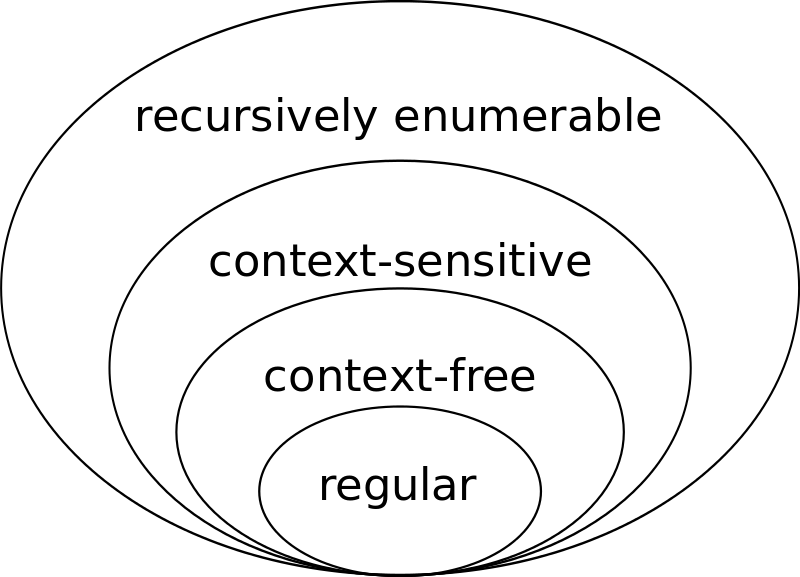
\includegraphics[width=0.8\textwidth]{images/chomsky-hierarchy}
    \newline
    \begin{center}
        {\tiny Image Source: \url{https://en.wikipedia.org/wiki/Chomsky_hierarchy}}
    \end{center}
\end{columns}
\end{frame}

\begin{frame}{Grammars for Programming Languages}
    \begin{itemize}[<+->]
        \item Recursively Enumerable (Type-0) grammars are generally
            too powerful to describe programming languages.  (They
            would also be too difficult to compile!)
        \item Most programming languages do contain at least a handful
            of context-sensitive attributes, though writing true
            context sensitive grammars is not needed in most cases.
        \item Context-Free (Type-2) grammars will be our focus.  Even
            in context-sensitive languages, the syntax is often
            expressed first as a context free grammar with additional
            constraints applied by the compiler.
        \item Regular Grammars are too limited to express general
            programming languages. They are typically useful for
            searching and general pattern matching.
    \end{itemize}
\end{frame}

\begin{frame}{Backus Naur Form (BNF)}
    \begin{itemize}[<+->]
        \item BNF is a metalanguage which describes context-free
            grammars.
        \item Invented by Naur, edited by Backus, first used to
            describe Algol-60.
        \item By far, BNF is the most popular metalanguage notation.
        \item BNF non-terminals are described using meaningful
            phrases enclosed in angle brackets $\langle \rangle$.
        \item Replacement arrows are $::=$ 
        \item Alternate replacements are separated with $|$.
        \item Terminal strings are enclosed in single quotes.
    \end{itemize}
\end{frame}

\begin{frame}{Example Grammar}
    \begin{grammar}
        <S> ::= <Expression>

        <Expression> ::= <Term> | <Expression> `+' <Term>

        <Term> ::= <Factor> | <Term> `*' <Factor>

        <Factor> ::= <Unit> | (<Expression>)

        <Unit> ::= `0'|`1'|`2'|`3'|`4'|`5'|`6'|`7'|`8'|`9'
    \end{grammar}
\end{frame}

\section{Ledgard}

\begin{frame}{The Ledgard Programming Language}
    \begin{itemize}[<+->]
        \item Ledgard is a teaching language.
        \item Designed by Lee Wittenberg in order to teach students
            how to write compilers.
        \item Named in honor of Henry Ledgard, author of 
            {\em Programming Language Landscapes}.
        \item Essentially contains ``just enough'' of the elements of
            programming languages to explore compiler creation.
    \end{itemize}
\end{frame}

\begin{frame}{Ledgard Syntax}
    \begin{grammar}
        <program> ::= `program' <decl-list> `begin' <stmt-list> `end' `;'

        <decl-list> ::= <declaration> | <decl-list> <declaration>

        <declaration> ::= <identifier-list> `:' <type> `;'

        <identifier-list> ::= <identifier> | <identifier-list> `,'
            <identifier>

        <type> ::= <simple-type> | <array-type>

        <simple-type> ::= `integer' | `boolean'

        <array-type> ::= `array' `[' <bounds> `]' `of' <type>

        <bounds> ::= <integer-literal> `..' <integer-literal>
    \end{grammar}
\end{frame}

\begin{frame}{Ledgard Syntax (continued)}
    \begin{grammar}
        <stmt-list> ::= <statement> | <stmt-list> <statement>

        <statement> ::= <assignment-stmt> | <exchange-stmt>
            | <if-stmt>  | <loop-stmt> | <input-stmt> | <output-stmt>

        <assignment-stmt> ::= <variable> `:=' <expression> `;'

        <exchange-stmt> ::= <variable> `:=:' <variable> `;'

        <if-stmt> ::= `if' <expression> `then' <stmt-list> `end' `if' `;'
            \alt `if' <expression> `then' <stmt-list> `else'
            <stmt-list> `end' `if' `;'

        <loop-stmt> ::= `while' <expression> `loop' <stmt-list> `end'
            `loop' `;'
    \end{grammar}
\end{frame}

\begin{frame}{Ledgard Syntax (continued)}
    \begin{grammar}
        <input-statement> ::= `input' <variable-list> `;'

        <output-statement> ::= `output' <variable-list> `;'

        <variable-list> ::= <variable> | <variable-list> `,'
            <variable>

        <expression> ::= <operand> | <operand> <operator> <operand>

        <operand> ::= <variable> | <integer-literal>
            | <boolean-literal> | `(' <expression> `)' |
            `not' <operand>

        <variable> ::= <variable> | <variable> `[' <expression> `]'
    \end{grammar}
\end{frame}

\begin{frame}{Ledgard Syntax (continued)}
    \begin{grammar}
        <boolean-literal> ::= `true' | `false'

        <operator> ::= `<' | `<=' | `==' | `<>' | `>=' | `>' |
          `+' | `-' | `*' | `/' | `and' | `or'
    \end{grammar}

    \begin{itemize}
        \item An integer-literal is just a string of digits 0-9.
        \item Comments begin with \texttt{--} and continue to the end
          of the line.
    \end{itemize}
\end{frame}

\end{document}


